\documentclass{beamer}

\usepackage[italian]{babel}
\usepackage[utf8]{inputenc}


\setbeamertemplate{caption}{\centering\insertcaption\par}

\title{I Frattali}

\author{Carlo Buccisano}
\date{Tesina Esame di Stato 2015-2016}
\institute{Liceo Scientifico F. Lussana}
\logo{\includegraphics[width=15mm]{"../Copertina/logo"}}

\usetheme{Marburg}
\useoutertheme[right]{sidebar}
\setbeamercovered{dynamic}

\begin{document}
	\section{Introduzione}
		\begin{frame}
			\begin{center}
				\includegraphics[width=0.5\textwidth]{"../Copertina/blue_lagoon"}
			\end{center}
			\maketitle
		\end{frame}
		\begin{frame}
			\frametitle{Piano della presentazione}
			\tableofcontents
		\end{frame}
		\begin{frame}
			\frametitle{Premessa}
			Perché ho scelto questa tesina?
			\begin{itemize}
				\item passione per la matematica e l'informatica
				\item i frattali sono un campo della matematica recente e interessante
				\item i frattali possono dare un'immagine diversa della matematica, spesso vista erroneamente come ostica e astratta
			\end{itemize}
		\end{frame}
	\section{Cos'è un frattale}
		\begin{frame}
			\frametitle{Cos'è un frattale}
			Un frattale è una particolare figura geometrica caratterizzata da:
			\begin{itemize}
				\item autosimilarità
				\item perimetro infinito o nullo
				\item area finita (o nulla)
				\item irregolarità
				\item dimensione non intera
			\end{itemize}
		\end{frame}
		\begin{frame}
			\frametitle{Cos'è un frattale}
			\framesubtitle{Autosimilarità}
			In geometria due poligoni sono detti simili se e solo se hanno angoli uguali e lati in proporzione. Per i frattali l'autosimilarità consiste nel fatto che una loro parte è simile al frattale di partenza.
			\bigskip
			\begin{columns}
				\begin{column}{0.5\textwidth}
					\begin{figure}[H]
						\centering
						\includegraphics[width=0.8\linewidth]{"../Varie/autosimilarita"}
						\caption{Autosimilarità nel triangolo di Sierpinski}
						\label{fig:autosimilarita}
					\end{figure}
				\end{column}
				\begin{column}{0.5\textwidth}
					\begin{figure}[h]
						\centering
						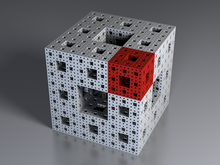
\includegraphics[width=0.5\linewidth]{../Varie/menger_autosimile}
						\caption{Autosimilarità nella spugna di Menger}
						\label{fig:mengerautosimile}
					\end{figure}

				\end{column}
			\end{columns}
		\end{frame}
		\begin{frame}
			\frametitle{Cos'è un frattale}
			\framesubtitle{Perimetro infinito o nullo}
			Spesso i frattali hanno perimetro infinito o nullo.
			Ad esempio la curva di Koch ha perimetro infinito: a ogni iterazione il perimetro diviene i $4/3$ del precedente quindi
			\begin{gather*}
				p = \lim_{n \rightarrow + \infty} \left(\frac{4}{3} \right)^n \cdot p_0 = + \infty
			\end{gather*}
			\begin{columns}
				\begin{column}{0.5\textwidth}
					\begin{figure}[h]
						\centering
						\includegraphics[width=0.5\linewidth]{"../Curva di Koch/koch"}
						\caption{Curva di Koch}
						\label{fig:curva_koch}
					\end{figure}
				\end{column}
				\begin{column}{0.5\textwidth}
					\begin{figure}[h]
						\centering
						\includegraphics[width=0.7\linewidth]{"../Curva di Koch/kochcolori"}
						\caption{Autosimilarità nella curva di Koch}
						\label{fig:koch_autosimile}
					\end{figure}
				\end{column}
			\end{columns}
		\end{frame}
		\begin{frame}
			\frametitle{Cos'è un frattale}
			\framesubtitle{Area finita o nulla}
			Nonostante i frattali possano avere perimetro infinito, la loro area sarà sempre finita o nulla.
			Ad esempio l'area del tappeto di Sierpinski è nulla mentre l'area del fiocco di Koch è finita e vale $\left( \frac{8}{5} \right) \cdot A_0$, dove $A_0$ è l'area del triangolo iniziale.
			\begin{columns}
				\begin{column}{0.5\textwidth}
					\begin{figure}[h]
						\centering
						\includegraphics[width=0.5\linewidth]{"../Tappeto di Sierpinski/tappeto_sierpinski"}
						\caption{Tappeto di Sierpinski}
						\label{fig:tappeto_sierpinski}
					\end{figure}
				\end{column}
				\begin{column}{0.5\textwidth}
					\begin{figure}[h]
						\centering
						\includegraphics[width=0.7\linewidth]{"../Fiocco di Koch/fioccodineve"}
						\caption{Fiocco di Koch}
						\label{fig:fiocco_koch}
					\end{figure}
				\end{column}
			\end{columns}
		\end{frame}
		\begin{frame}
			\frametitle{Cos'è un frattale}
			\framesubtitle{Irregolarità}
			Un frattale non può essere definito come luogo di punti che soddisfino certe condizioni geometriche o analitiche, perché per descriverlo si utilizzano definizioni ricorsive.
			\begin{figure}[h]
				\centering
				\includegraphics[width=0.7\linewidth]{"../Triangolo di Sierpinski/sierpinski_triangle_algo"}
				\caption{Snippet Python per generare il triangolo di Sierpinski}
				\label{fig:sierpinskitrianglealgo}
			\end{figure}

		\end{frame}
		\begin{frame}
			\frametitle{Cos'è un frattale}
			\framesubtitle{Dimensione non intera}
			La dimensione frattale è stata introdotta da Hausdorff ed è definita come:
			\begin{gather*}
			D_f = \frac{\log N}{\log ( 1 / K )}
			\end{gather*}
			dove $N$ è il numero di parti simili in cui il frattale può essere diviso e $K$ è il rapporto di omotetia.
			\begin{block}{Esempi}
				La spugna di Menger ha dimensione $\frac{\log20}{\log3} \approx 2.7268$\\
				Il triangolo di Sierpinski ha dimensione $\frac{\log3}{\log2} \approx 1.585$
			\end{block}
		\end{frame}
	\section{Tipi di frattali}
		\begin{frame}
			\frametitle{Tipi di frattali}
			Si distinguono:
			\begin{itemize}
				\item frattali deterministici
				\item frattali aleatori
			\end{itemize}
			\bigskip
			A seconda di come vengono generati al calcolatore poi vi sono:
			\begin{itemize}
				\item frattali IFS
				\item frattali LS
			\end{itemize}
		\end{frame}
		\begin{frame}
			\frametitle{Tipi di frattali}
			\framesubtitle{Frattali IFS}
			I frattali IFS (\textit{Iterated Function System}) vengono generati a partire da un insieme di punti nel piano a cui vengono applicate trasformazioni geometriche in sequenza. Quando le successive immagini convergono si parla di frattale IFS.\\
			Un frattale IFS, generato tramite affinità, è la curva di Koch.
			\begin{columns}
				\begin{column}{0.25\textwidth}
					\begin{center}
						\includegraphics[width=1\linewidth]{"../Curva di Koch/t1"}
					\end{center}
				\end{column}
				\begin{column}{0.25\textwidth}
					\begin{center}
						\includegraphics[width=1\linewidth]{"../Curva di Koch/t2"}
					\end{center}
				\end{column}
				\begin{column}{0.25\textwidth}
					\begin{center}
						\includegraphics[width=1\linewidth]{"../Curva di Koch/t3"}
					\end{center}
				\end{column}
				\begin{column}{0.25\textwidth}
					\begin{center}
						\includegraphics[width=1\linewidth]{"../Curva di Koch/t4"}
					\end{center}
				\end{column}
			\end{columns}
		\end{frame}
		\begin{frame}
			\frametitle{Tipi di frattali}
			\framesubtitle{Frattali LS}
			Un frattale LS (\textit{Lindenmayer System}) non è propriamente autosimile, in quanto non è possibile suddividere la figura in un certo numero di parti simili ad essa. \`E però possibile suddividere il frattale in un numero \emph{finito} di frattali IFS. Un esempio è il fiocco di Koch, non autosimile, ma divisibile in un numero finito di frattali IFS (curve di Koch).
			\bigskip
			\begin{columns}
				\begin{column}{0.5\textwidth}
					\begin{center}
						\includegraphics[width=0.8\linewidth]{"../Fiocco di Koch/fiocco"}
					\end{center}
				\end{column}
				\begin{column}{0.5\textwidth}
					\begin{tiny}
						 Assioma: \textbf{F- -F- -F} (un triangolo equilatero)\\
						 Angolo: $60$ gradi \\
						 Fattore omotetia: $3$\\  
						 Legge: \textbf{F} $\to$ \textbf {F+F- -F+F}
					\end{tiny}
				\end{column}
			\end{columns}
		\end{frame}
	\section{Frattali in natura}
		\begin{frame}
			\frametitle{Frattali in natura}
			In natura si trovano moltissimi esempi di oggetti il cui schema sembra essere molto più aderente alla geometria frattale rispetto a quella euclidea, i cosiddetti \textit{frattali biomorfi}.
			\bigskip
			\begin{columns}
				\begin{column}{0.25\textwidth}
					\begin{center}
						\includegraphics[width=1\linewidth]{"../Frattali in natura/ammoniti"}
					\end{center}
				\end{column}
				\begin{column}{0.25\textwidth}
					\begin{center}
						\includegraphics[width=1\linewidth]{"../Frattali in natura/Fractal_Broccoli"}
					\end{center}
				\end{column}
				\begin{column}{0.25\textwidth}
					\begin{center}
						\includegraphics[width=1\linewidth]{"../Frattali in natura/intense-fulminazioni"}
					\end{center}
				\end{column}
				\begin{column}{0.25\textwidth}
					\begin{center}
						\includegraphics[width=1\linewidth]{"../Frattali in natura/fiore"}
					\end{center}
				\end{column}
			\end{columns}
		\end{frame}
	\section{Applicazioni dei frattali}
		\begin{frame}
			\frametitle{Applicazioni dei frattali}
			I frattali trovano numerose applicazioni, ad esempio:
			\begin{itemize}
				\item moto di fluidi turbolenti o fenomeni di combustione
				\item compressione di video e immagini
				\item studio della natura: dalle linee di costa, ai corsi dei fiumi e alle catene montuose
				\item percolazione, cioé lento movimento di un fluido su un materiale poroso
			\end{itemize} 
			\begin{columns}
				\begin{column}{0.5\textwidth}
					\begin{center}
						\includegraphics[width=0.7\linewidth]{"../Frattali in natura/coast"}
					\end{center}
				\end{column}
				\begin{column}{0.5\textwidth}
					\begin{center}
						\includegraphics[width=0.7\linewidth]{"../Frattali in natura/river"}
					\end{center}
				\end{column}
			\end{columns}
		\end{frame}
	\section{Frattali famosi}
		\subsection{Insieme di Cantor}
			\begin{frame}
				\frametitle{Insieme di Cantor}
					L'insieme di Cantor è un sottoinsieme dell'intervallo $[0, 1]$ dei numeri reali.
					L'algoritmo che lo genera è il seguente:
					\begin{enumerate}
						\item si divide l'intervallo in tre parti congruenti
						\item si rimuove il segmento centrale aperto (dunque i due estremi non vengono rimossi), ottenendo così due intervalli (chiusi) più piccoli
						\item si riapplica il punto 1. ai due intervalli ottenuti
					\end{enumerate}
					\begin{center}
						\includegraphics[width=0.9\linewidth]{"../Insieme di Cantor/cantor_set_in_seven_iterations"}
					\end{center}

			\end{frame}
			\begin{frame}
				\frametitle{Insieme di Cantor}
				\framesubtitle{Perimetro e dimensione}
				Ad ogni passo viene rimosso un terzo del numero di punti (ogni intervallo diventa i $2/3$ del precedente) dunque il perimetro finale del frattale è:
				\begin{gather*}
				p = \lim_{n \to +\infty} \left( \frac{2}{3} \right) ^ n \cdot 1 = 0
				\end{gather*}
				Ad ogni iterazione, ogni intervallo viene diviso in due parti simili al frattale stesso, con fattore di omotetia $K=1/3$ dunque la sua dimensione di Hausdorff è:
				\begin{gather*}
				D_f = \frac{\log 2}{\log 3} \approx 0.6309
				\end{gather*}
			\end{frame}
			\begin{frame}
				\frametitle{Insieme di Cantor}
				\framesubtitle{Cardinalità}
				La cardinalità dell'insieme di Cantor è la stessa dell'intervallo $[0, 1]$ e, quindi, dei reali.\\
				Infatti all'$n$-esima iterazione  vengono rimossi tutti i numeri che, nella loro scrittura decimale in base $3$, hanno la cifra $1$ nell'$n$-esima posizione. In generale solo i punti scrivibili con le cifre $0$ e $2$, in base $3$,  appartengono all'insieme. Trasformando i $2$ in $1$ e leggendo i numeri in binario si ottiene di nuovo tutto l'intervallo $[0, 1]$, da cui deriva la stessa cardinalità.
				\begin{columns}
					\begin{column}{0.5\textwidth}
						\begin{center}
							\includegraphics[width=0.5\linewidth]{"../Insieme di Cantor/Cantor_dust"}
						\end{center}
					\end{column}
					\begin{column}{0.5\textwidth}
						\begin{center}
							\includegraphics[width=0.5\linewidth]{"../Insieme di Cantor/3D_Cantor_set"}
						\end{center}
					\end{column}
				\end{columns}
			\end{frame}
		\subsection{Insieme di Mandelbrot}
			\begin{frame}
				\frametitle{Insieme di Mandelbrot}
				\framesubtitle{Definizione}
				L'insieme di Mandelbrot è costituito da tutti i numeri complessi $c$ tali che che la successione\\\bigskip
				$
				\begin{cases}
				z_0 = 0 \\
				z_n = z_{n-1}^2 + c 
				\end{cases}
				$
				\\\bigskip
				è limitata superiormente.
				\begin{center}
					\includegraphics[width=0.5\linewidth]{"../Insieme di Mandelbrot/Mandelset_hires"}
				\end{center}
			\end{frame}
			\begin{frame}
				\frametitle{Insieme di Mandelbrot}
				\framesubtitle{Escape Time Algorithm}
				Per ogni pixel $(x, y)$, che rappresenta il numero complesso $c = x + i y$, viene calcolato se e quanto velocemente diverge $z_n$ e, in base al risultato ottenuto, viene assegnato un colore al pixel.
				Chiaramente, per evitare loop infiniti, viene fissata una soglia oltre la quale si ferma il calcolo di $z_n$ e si ipotizza che la successione non diverge. 
				\begin{columns}
					\begin{column}{0.5\textwidth}
						\begin{center}
							\includegraphics[width=0.7\linewidth]{"../Insieme di Mandelbrot/mandelbrot_schifo"}
						\end{center}
					\end{column}
					\begin{column}{0.5\textwidth}
						\begin{center}
							\includegraphics[width=0.7\linewidth]{"../Insieme di Mandelbrot/Escape_Time_Algorithm_bands"}
						\end{center}
					\end{column}
				\end{columns}
			\end{frame}
			\begin{frame}
				\frametitle{Insieme di Mandelbrot}
				\framesubtitle{Continuous Smooth Coloring}
				L'algoritmo, per ogni numero complesso $c$ per cui $z_n$ diverge, calcola il primo indice $N$ per cui $|z_N| > 2$ e ritorna un numero reale $v$, in base a cui è deciso il colore del pixel, calcolato come:
				\begin{gather*}
				v = N - \log_2(\log_2|z_N|)
				\end{gather*}
				\begin{figure}[h]
					\centering
					\includegraphics[width=1\linewidth]{"../Insieme di Mandelbrot/smooth"}
					\caption{Snippet C++}
					\label{fig:smooth}
				\end{figure}
			\end{frame}
			\begin{frame}
				\frametitle{Insieme di Mandelbrot}
				\framesubtitle{Supersampling}
				L'algoritmo consiste nella costruzione di una nuova immagine, a dimensioni ridotte, dove ogni pixel ha colore pari alla media dei colori di un quadrato $N \times N$ di punti dell'immagine originale. In questo modo gli \textit{outliers} vengono praticamente eliminati.
				\begin{figure}[h]
					\centering
					\includegraphics[width=0.8\linewidth]{"../Insieme di Mandelbrot/supersampling"}
					\caption{Snippet C++}
					\label{fig:supersampling}
				\end{figure}

			\end{frame}
			\begin{frame}
				\frametitle{Insieme di Mandelbrot}
				\framesubtitle{Alcune immagini}
				\begin{center}
					\includegraphics[width=0.7\linewidth]{"../Insieme di Mandelbrot/z1"}
				\end{center}
			\end{frame}
			\begin{frame}
				\frametitle{Insieme di Mandelbrot}
				\framesubtitle{Alcune immagini}
				\begin{center}
					\includegraphics[width=0.7\linewidth]{"../Insieme di Mandelbrot/z2"}
				\end{center}
			\end{frame}
			\begin{frame}
				\frametitle{Insieme di Mandelbrot}
				\framesubtitle{Alcune immagini}
				\begin{center}
					\includegraphics[width=0.7\linewidth]{"../Insieme di Mandelbrot/detail5"}
				\end{center}
			\end{frame}
			\begin{frame}
				\frametitle{Insieme di Mandelbrot}
				\framesubtitle{Alcune immagini}
				\begin{center}
					\includegraphics[width=0.7\linewidth]{"../Insieme di Mandelbrot/detail6"}
				\end{center}
			\end{frame}
			\begin{frame}
				\frametitle{Insieme di Mandelbrot}
				\framesubtitle{Alcune immagini}
				\begin{center}
					\includegraphics[width=0.7\linewidth]{"../Insieme di Mandelbrot/z5"}
				\end{center}
			\end{frame}
			\begin{frame}
				\frametitle{Insieme di Mandelbrot}
				\framesubtitle{Alcune immagini}
				\begin{center}
					\includegraphics[width=0.7\linewidth]{"../Insieme di Mandelbrot/z7"}
				\end{center}
			\end{frame}
			\begin{frame}
				\frametitle{Insieme di Mandelbrot}
				\framesubtitle{Alcune immagini}
				\begin{center}
					\includegraphics[width=0.7\linewidth]{"../Insieme di Mandelbrot/z8"}
				\end{center}
			\end{frame}
			\begin{frame}
				\frametitle{Insieme di Mandelbrot}
				\framesubtitle{Alcune immagini}
				\begin{center}
					\includegraphics[width=0.7\linewidth]{"../Insieme di Mandelbrot/z9"}
				\end{center}
			\end{frame}
			\begin{frame}
				\frametitle{Insieme di Mandelbrot}
				\framesubtitle{Alcune immagini}
				\begin{center}
					\includegraphics[width=0.7\linewidth]{"../Insieme di Mandelbrot/z10"}
				\end{center}
			\end{frame}
			\begin{frame}
				\frametitle{Insieme di Mandelbrot}
				\framesubtitle{Alcune immagini}
				\begin{center}
					\includegraphics[width=0.7\linewidth]{"../Insieme di Mandelbrot/z13"}
				\end{center}
			\end{frame}
			\begin{frame}
				\frametitle{Insieme di Mandelbrot}
				\framesubtitle{Alcune immagini}
				\begin{center}
					\includegraphics[width=0.7\linewidth]{"../Insieme di Mandelbrot/z14"}
				\end{center}
			\end{frame}
			\begin{frame}
				\frametitle{Insieme di Mandelbrot}
				\framesubtitle{Alcune immagini}
				\begin{center}
					\includegraphics[width=0.7\linewidth]{"../Insieme di Mandelbrot/z15"}
				\end{center}
			\end{frame}
		\subsection{Insieme di Julia}
			\begin{frame}
				\frametitle{Insieme di Julia}
				\framesubtitle{Definizione}
				L'insieme di Julia di una funzione complessa $f$, indicato come $J(f)$, è definito come l'insieme di tutti i numeri complessi tali che il comportamento della funzione in seguito a ripetute iterazioni è caotico, ovvero in seguito ad una piccola perturbazione varia drasticamente. 	Un interessante insieme di Julia è quello relativo alla funzione complessa $f_c(z) = z^2 + c$ dove $z$ è un numero complesso e $c$ una costante. 
				% IMMAGINI %
			\end{frame}
			\begin{frame}
				\frametitle{Insieme di Julia}
				\framesubtitle{Alcune immagini}
				\begin{center}
					\includegraphics[width=0.7\linewidth]{"../Insieme di Julia/cosa44_2"}
				\end{center}
			\end{frame}
			\begin{frame}
				\frametitle{Insieme di Julia}
				\framesubtitle{Alcune immagini}
				\begin{center}
					\includegraphics[width=0.7\linewidth]{"../Insieme di Julia/cosa48"}
				\end{center}
			\end{frame}
			\begin{frame}
				\frametitle{Insieme di Julia}
				\framesubtitle{Alcune immagini}
				\begin{center}
					\includegraphics[width=0.7\linewidth]{"../Insieme di Julia/cosa55"}
				\end{center}
			\end{frame}
			\begin{frame}
				\frametitle{Insieme di Julia}
				\framesubtitle{Alcune immagini}
				\begin{center}
					\includegraphics[width=0.7\linewidth]{"../Insieme di Julia/cosa58"}
				\end{center}
			\end{frame}
			\begin{frame}
				\frametitle{Insieme di Julia}
				\framesubtitle{Alcune immagini}
				\begin{center}
					\includegraphics[width=0.7\linewidth]{"../Insieme di Julia/cosa63"}
				\end{center}
			\end{frame}
			\begin{frame}
				\frametitle{Insieme di Julia}
				\framesubtitle{Alcune immagini}
				\begin{center}
					\includegraphics[width=0.7\linewidth]{"../Insieme di Julia/julia1"}
				\end{center}
			\end{frame}
			\begin{frame}
				\frametitle{Insieme di Julia}
				\framesubtitle{Alcune immagini}
				\begin{center}
					\includegraphics[width=0.7\linewidth]{"../Insieme di Julia/julia2"}
				\end{center}
			\end{frame}
			\begin{frame}
				\frametitle{Insieme di Julia}
				\framesubtitle{Alcune immagini}
				\begin{center}
					\includegraphics[width=0.7\linewidth]{"../Insieme di Julia/julia4"}
				\end{center}
			\end{frame}
			\begin{frame}
				\frametitle{Insieme di Julia}
				\framesubtitle{Alcune immagini}
				\begin{center}
					\includegraphics[width=0.7\linewidth]{"../Insieme di Julia/julia6"}
				\end{center}
			\end{frame}
			\begin{frame}
				\frametitle{Insieme di Julia}
				\framesubtitle{Alcune immagini}
				\begin{center}
					\includegraphics[width=0.7\linewidth]{"../Insieme di Julia/julia8"}
				\end{center}
			\end{frame}
			\begin{frame}
				\frametitle{Insieme di Julia}
				\framesubtitle{Alcune immagini}
				\begin{center}
					\includegraphics[width=0.7\linewidth]{"../Insieme di Julia/cosa52"}
				\end{center}
			\end{frame}
	\section{James Joyce}
		\begin{frame}
			\frametitle{James Joyce}
			\framesubtitle{Life and Works}
			\begin{center}
				\includegraphics[width=0.4\linewidth]{"../Inglese - Joyce/james-joyce"}
			\end{center}
			James Joyce (1882 - 1941) was an Irish novelist and poet. He is considered one of the most influential authors of the twentieth century.\\
			Joyce's charateristic narrative mode is the so called \textit{stream of consciousness}, which attempts to give the written equivalent of the character's thought processes. 
		\end{frame}
		\begin{frame}
			\frametitle{James Joyce}
			\framesubtitle{Finnegans Wake}
			Finnegans Wake is the last book by James Joyce, published in 1939, two years before the author's death. It is certainly the most ``difficult'' book, among Joyce' ones.
			\begin{center}
				\includegraphics[width=0.6\linewidth]{"../Inglese - Joyce/finnegans_scheme"}
			\end{center}
		\end{frame}
		\begin{frame}
			\frametitle{James Joyce}
			\framesubtitle{Multifractal Structure of Finnegans Wake}
			Scientists found that the variations of sentence lengths were governed by a the dynamics of a cascade, meaning their construction is a fractal, characterized by self-similarity. Finnegans Wake, the scientists found, was the most complex of all.
			\begin{center}
				\includegraphics[width=0.7\linewidth]{"../Inglese - Joyce/fractal_graphic"}
			\end{center}

		\end{frame}
	\section{Eterno ritorno dell'uguale}
		\begin{frame}
			\frametitle{Eterno ritorno dell'uguale}
			\begin{center}
				\includegraphics[width=0.2\linewidth]{../Nietzsche/Nietzsche187a}
			\end{center}
			\begin{quotation}
				``Tutto va, tutto torna indietro; eternamente ruota la ruota dell'essere. Tutto muove, tutto torna a fiorire, eternamente corre l'anno dell'essere. Tutto crolla, tutto viene di nuovo connesso; eternamente l'essere si costruisce la medesima abitazione. Tutto si diparte, tutto torna a salutarsi; eternamente fedele a se stesso rimane l'anello dell'essere. In ogni attimo comincia l'essere; attorno ad ogni 'qui' ruota la sfera del 'là'. Il centro è dappertutto. Ricurvo è il sentiero dell'eternità.''
			\end{quotation}
			
		\end{frame}
		\begin{frame}
			\frametitle{Eterno ritorno dell'uguale}
			\framesubtitle{Concezione ciclica del tempo}
			Nietzsche, con la teoria dell'eterno ritorno, recupera una concezione precristiana del mondo, presente nella Grecia presocratica e nelle antiche civiltà indiane, in cui vi è una visione ciclica del tempo, opposta a quella rettilinea di tipo cristiano-moderna.
			Secondo Nietzsche, solo grazie ad una concezione ciclica del tempo, si può giungere ad una vera felicità.
			\begin{center}
				\includegraphics[width=0.4\linewidth]{../Nietzsche/Ouroboros}
			\end{center}

		\end{frame}
		\begin{frame}
			\frametitle{Eterno ritorno dell'uguale}
			\framesubtitle{Interpretazioni}
			\begin{itemize}
				\item potrebbe trattarsi di una \textbf{certezza cosmologica}, come talvolta afferma Nietzsche stesso, dal momento che la quantità di energia nell'universo è finita e il tempo infinito e quindi le manifestazioni e le combinazioni del mondo sono prima o poi destinate a ripetersi
				\item potrebbe invece essere un'\textbf{ipotesi sull'essere} che funge da imperativo categorico, che prescrive di amare la vita e agire come se tutto dovesse ritornare
				\item oppure potrebbe essere l'\textbf{enunciazione metaforica di un modo di essere dell'essere}, che l'uomo può incarnare solo nella misura in cui accetta la vita.
			\end{itemize}
		\end{frame}
		
\end{document}